
%(BEGIN_QUESTION)
% Copyright 2007, Tony R. Kuphaldt, released under the Creative Commons Attribution License (v 1.0)
% This means you may do almost anything with this work of mine, so long as you give me proper credit

Regn ut høyden med glyserin ($\rho=1259kg/m³$) i et vertikalt rør om det er et hydrostatisk trykk på 1.5 Bar i bunn av røret:

$$\includegraphics[height=6cm]{i02951x01.eps}$$

Glyserin høyde = \underbar{\hskip 50pt} meter 

\vskip 30pt

Regn også ut høyden med castor olje ($\rho=961/m³$) som skal til for å genere det samme hydrostatiske trykket:

\vskip 10pt

Castor olje høyde =  \underbar{\hskip 50pt} meter

\underbar{file i02951}
%(END_QUESTION)





%(BEGIN_ANSWER)

Glycerine height = \underbar{\bf 12.14} meter

\vskip 10pt

Castor oil height = \underbar{\bf 15.91} meter

%(END_ANSWER)





%(BEGIN_NOTES)

%INDEX% Physics, static fluids: hydrostatic pressure

%(END_NOTES)


